%!TEX program = xelatex
\documentclass{beamer}
\usepackage{ctex, hyperref}
\usepackage[T1]{fontenc}

% other packages
\usepackage{latexsym,amsmath,xcolor,multicol,booktabs,calligra}
\usepackage{graphicx,pstricks,listings,stackengine}

\author{吴亚伦}
\title{Sphinx: Enabling Privacy-Preserving Online Learning over the Cloud}
\subtitle{分享在Sphinx论文中的一些思考、理解、推理、质疑和求证}
\institute{北京交通大学·网络空间安全}
\date{2023年03月24日}
\usepackage{bjtu}

% defs
\def\cmd#1{\texttt{\color{red}\footnotesize $\backslash$#1}}
\def\env#1{\texttt{\color{blue}\footnotesize #1}}
\definecolor{deepblue}{rgb}{0,0,0.5}
\definecolor{deepred}{rgb}{0.6,0,0}
\definecolor{deepgreen}{rgb}{0,0.5,0}
\definecolor{halfgray}{gray}{0.55}

\lstset{
    basicstyle=\ttfamily\small,
    keywordstyle=\bfseries\color{deepblue},
    emphstyle=\ttfamily\color{deepred},    % Custom highlighting style
    stringstyle=\color{deepgreen},
    numbers=left,
    numberstyle=\small\color{halfgray},
    rulesepcolor=\color{red!20!green!20!blue!20},
    frame=shadowbox,
}



\begin{document}
\kaishu
% 每页根据frame标签来分割
\begin{frame}
    \titlepage
    \begin{figure}[htpb]
        \begin{center}
            
\includegraphics[width=0.2\linewidth]{pic/bjtu_logo.jpeg}
        \end{center}
    \end{figure}
\end{frame}


% 目录页
\begin{frame}
%tableofcontents 自动生成目录
    \tableofcontents[sectionstyle=show,subsectionstyle=show/shaded/hide,subsubsectionstyle=show/shaded/hide]
\end{frame}


% 第一章
\section{课前讨论}
\subsection{思考:机器学习与隐私保护}
\begin{frame}{机器学习与隐私保护}
	\begin{exampleblock}{思考以下问题:(互动讨论,5-10分钟)}
    \begin{itemize}[<+-| alert@+>]
        \item 1.为什么研究机器学习的隐私保护?不做隐私保护会有什么危害吗?
        \item 2.机器学习的隐私保护,保护对象是谁? 
        \item 3.你平时进行机器学习实验的时候会进行隐私保护吗?(如果有,则讲述如何进行保护的?如果没有,阐明原因。)
    \end{itemize}
    \end{exampleblock}
\end{frame}

\subsection{浅谈:MLaaS的演变历程}
\begin{frame}{MLaaS的演变历程}
	\begin{exampleblock}{从零开始搭建机器学习模型的4个步骤:}
    \begin{itemize}[<+-| alert@+>]
        \item 1.首先需要选择一个服务器/工作站(考虑CPU、显卡、主板、内存、硬盘)
        \item 2.安装服务器的系统软件(安装CentOS、Ubuntu或者Windows等,俗称“装机”)
        \item 3.安装服务器的应用软件(安装Anaconda、Python、CUDA、PyTorch等,俗称“搭环境”)
        \item 4.编写或复现机器学习模型代码,运行。
    \end{itemize}
    \end{exampleblock}
\end{frame}

\begin{frame}{MLaaS的演变历程}
	\begin{exampleblock}{第一阶段:基本方法/传统方法}
    \begin{itemize} %[<+-| alert@+>]
    	\item 方案介绍:按部就班的四步走。
    	\item 操作步骤:
    		\begin{itemize}
				\item 1.买服务器/工作站(买买买)。
				\item 2.安装系统软件(“装机”)
				\item 3.安装应用软件(“搭环境”)
				\item 4.编写或复现机器学习代码,运行。
			\end{itemize}
    	\item 存在问题:
    	\begin{itemize}
			\item 1.成本高,需要一次性购置设备(目前一台低配的工作站约需3~5万)
			\item 2.部署慢,需要装机装系统、还需要安装基础的应用软件,很繁琐。
       	\end{itemize}
    \end{itemize}
    \end{exampleblock}
\end{frame}

\begin{frame}{MLaaS的演变历程}
	\begin{exampleblock}{第二阶段:基础设施即服务(Infrastructure as a Service, IaaS)}
    \begin{itemize} %[<+-| alert@+>]
    	\item 方案介绍:商家提供云服务器和系统软件(Ubuntu/CentOS等)基础设施的“租赁”服务,按时长收费。
    	\item 提出背景:
    		\begin{itemize}
				\item 传统方法购买设备成本高=>IaaS从“买”变“租”,降低短期成本。
				\item 传统方法系统软件部署慢=>IaaS提供服务,支持任意系统一键安装。
			\end{itemize}
		\item 典型产品:阿里云、腾讯云(提供云主机、云存储)
    	\item 存在问题:
    	\begin{itemize}
			\item 尽管解决了设备购置成本高、系统软件部署慢的问题,但是应用软件(Anaconda、Python、CUDA、PyTorch等)的部署,也是一个很繁琐的过程。
       	\end{itemize}
    \end{itemize}
    \end{exampleblock}
\end{frame}

\begin{frame}{MLaaS的演变历程}
	\begin{exampleblock}{第三阶段:平台即服务(Platform as a Service, PaaS)}
    \begin{itemize} %[<+-| alert@+>]
    	\item 方案介绍:商家除了提供云服务器和系统软件(Ubuntu、CentOS等)之外,还提供Anaconda、CUDA、PyTorch等应用环境的安装。
    	\item 提出背景:
    		\begin{itemize}
				\item Iaas应用软件部署慢=>PaaS支持自定义软件镜像,一键安装开发环境。
			\end{itemize}
		\item 典型产品:Google Colab、AutoDL(提供算力租赁服务)
    	\item 存在问题:
    	\begin{itemize}
			\item 尽管具有成本低、系统软件部署快、应用软件部署的特点,但美中不足的是:机器学习模型复现遇到了困难(对于非专业人士很不友好,考虑“能不能不写代码就能用?”)。
       	\end{itemize}
    \end{itemize}
    \end{exampleblock}
\end{frame}

\begin{frame}{MLaaS的演变历程}
	\begin{exampleblock}{第四阶段:软件即服务(Software as a Service, SaaS)}    \begin{itemize} %[<+-| alert@+>]
    	\item 方案介绍:商家直接提供全套服务:服务器到位了、系统搭建了、环境配好了、模型搞定了,用户直接使用就可以了。
    	\item 提出背景:
    		\begin{itemize}
				\item PaaS模型复现困难=>SaaS直接提供全套服务。
			\end{itemize}
		\item 典型产品:谷歌云机器学习引擎、Amazon ML
    	\item 存在问题:虽然已经尽最大可能方便了用户,但还是觉得不够完美:面对众多模型,商家如何一一提供?
    \end{itemize}
    \end{exampleblock}
\end{frame}

\begin{frame}{MLaaS的演变历程}
	\begin{exampleblock}{第五阶段:机器学习即服务(Machine Learning as a Service, MLaaS)}
    \begin{itemize} %[<+-| alert@+>]
    	\item 个人理解:首先MLaaS是SaaS在机器学习领域的一种应用;其次MLaaS对SaaS进行改进了,引入了第三方(除了商家和用户之外的第三方)。这有点像消费者、京东自营和京东非自营三者之间的关系。
    	\item 典型产品:谷歌云机器学习引擎、Amazon ML
    \end{itemize}
    \end{exampleblock}
\end{frame}

\begin{frame}{MLaaS的演变历程}
	传统方法->IaaS->PaaS->SaaS->MLaaS的演变过程
	\begin{exampleblock}{优点:}
    \begin{itemize} %[<+-| alert@+>]
    	\item 部署速度越来越快;成本越来越低。
    \end{itemize}
    \end{exampleblock}
    \begin{exampleblock}{缺点:}
    \begin{itemize} %[<+-| alert@+>]
    	\item 一方(指:自己)->两方(指:云服务商和自己)->三方(指:云服务商、第三方模型提供者和自己):隐私安全性越来越低,因此:隐私保护问题不得不被考虑。
    \end{itemize}
    \end{exampleblock}
\end{frame}

%\subsection{简述:模型与数据的重要性}
%\begin{frame}{模型与数据的重要性}
%	假设现在有一组数据,班级同学以往的学习时间$x$和对应的考试分数$y$,想训练一个模型$f(x)$,根据未来学习的时间,预测考试分数$y^$。
%\end{frame}


%%%%%%%%%%%%%%%%%%%%%%%%%%%%%%%%%%%%%%%%%%%%%%%%%%%%%%%%%%%%%%%%%%%%%%%%%%%%%%%%
% 第二章
\section{论文概述}
\subsection{论文基本信息}
\begin{frame}{论文基本信息}
%论文封面	
	\begin{figure}[h]
    	\centering
        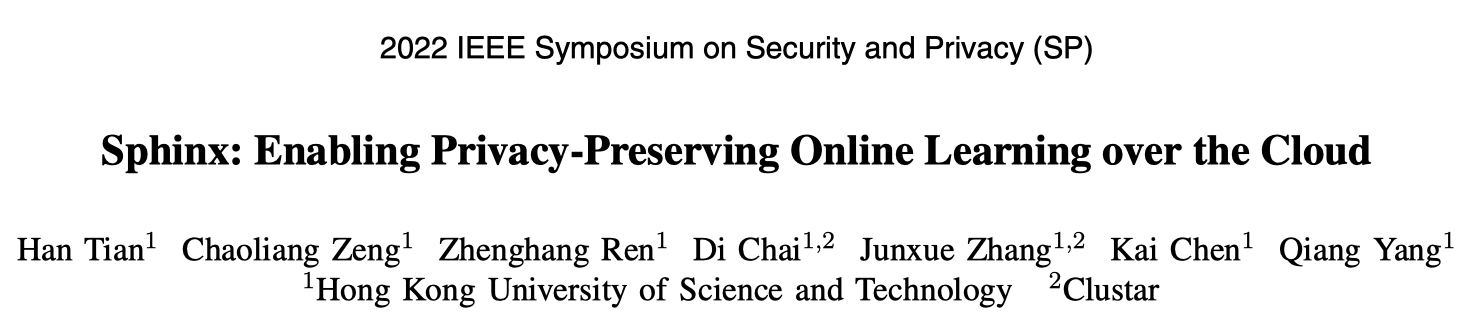
\includegraphics[height=.3\textheight]{pic/title.png}
    \end{figure} 
%分析介绍
	\begin{itemize}
        \item 题目:Sphinx: Enabling Privacy-Preserving Online Learning over the Cloud(Sphinx:实现云端保护隐私的在线学习)
        \item 会议:2022 IEEE Symposium on Security and Privacy (SP)
        \item 团队:香港科技大学团队 \& 星云(Clustar)
        \item 定位:是一篇使用同态加密(CKKS)和差分隐私进行隐私保护的文章(偏应用)。
    \end{itemize}
\end{frame}
\begin{frame}{论文基本信息}
	\begin{exampleblock}{学术团队/核心作者:}
	\begin{itemize}
        \item 星云(Clustar):深圳致星科技有限公司,注于高性能通用AI算力、隐私计算算力、网络算力的研发与场景应用,官网地址:\url{https://www.clustarai.com/}
        \item 陈凯:星云创始人、香港科大-微信人工智能技术联合实验室任、智能网络与系统实验室主任;研究方向:大数据和人工智能底层系统、隐私计算等。
        \item 张骏雪:星云联合创始人\&CTO、香港科大博士生;研究方向:数据挖掘、联邦学习、网络安全等。
    	\end{itemize}
    \end{exampleblock}
\end{frame}


\subsection{论文内容与贡献}
\begin{frame}{论文内容与贡献}
	\begin{itemize}[<+-| alert@+>]
		\item 提出了Sphinx,第一个考虑训练和推理两阶段的一个高效和隐私保护的在线深度学习系统。
		\item 将神经网络中的线性层分成了两部分,分别使用了不同的加密协议,并从理论和实验的角度进行了验证。(使用同态加密加密所有的偏置分量$b$、使用差分隐私扰乱线性分量$\omega$)。
%		\item 为了加速同态加密方案下的训练过程,Sphinx进行了多项优化(一方面通过刻意设计梯度、特征和模型参数之间的同态算数运算行为,减少了重缩放、重线性化的操作;另一方面Sphinx加速了加密操作,降低了客户端和服务器之间的通信时间)。
		\item 巧妙运用了CKKS的一些特性,加速了训练过程;在推理阶段引入了预处理过程,加速了推理效率、减小了通信开销。
	\end{itemize}
\end{frame}

%\subsection{插曲:为什么选择了这篇文章?}
\begin{frame}{小插曲:为什么选择了这篇文章?}
%论文封面	
	\begin{figure}[h]
    	\centering
        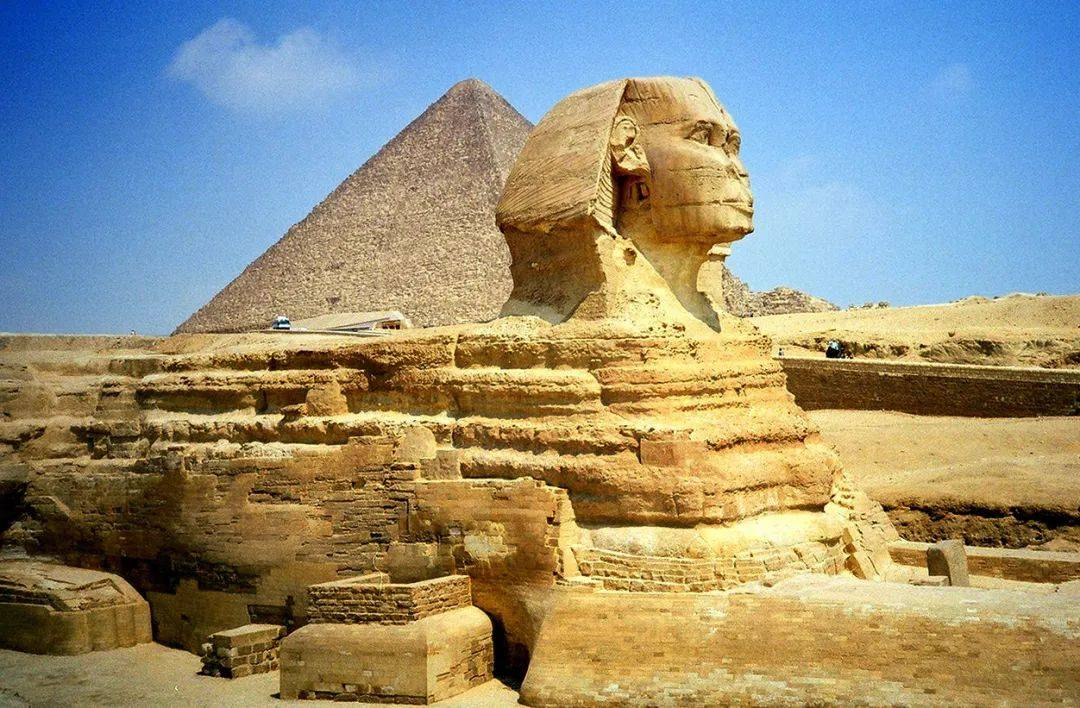
\includegraphics[height=.3\textheight]{pic/sphinx.jpeg}
    \end{figure} 
%分析介绍
	\begin{itemize}
        \item \small {很多论文都是A:B的结构,比如:“DLFuzz: Differential Fuzzing Testing of Deep Learning Systems”、“TensorFuzz: Debugging Neural Networks with Coverage-Guided Fuzzing”、“Deepsafe: A data-driven approach for checking adversarial robustness in neural networks”,被论文的题目吸引了。}
        \item \small {{\color {blue} 推理:之所以起名叫“Sphinx”,是因为本论文中神经网络中的偏置单元$b$和线性单元$\omega$用了不同的加密协议(有“狮身人面”内味了)。}}
%        \item 著名的狮身人面像金字塔,就是胡夫的儿子哈夫拉按照斯芬克斯的形象建造的金字塔。
    \end{itemize}
\end{frame}




\subsection{论文组织结构}
\begin{frame}{论文组织结构}
	\begin{figure}[h]
    	\centering
        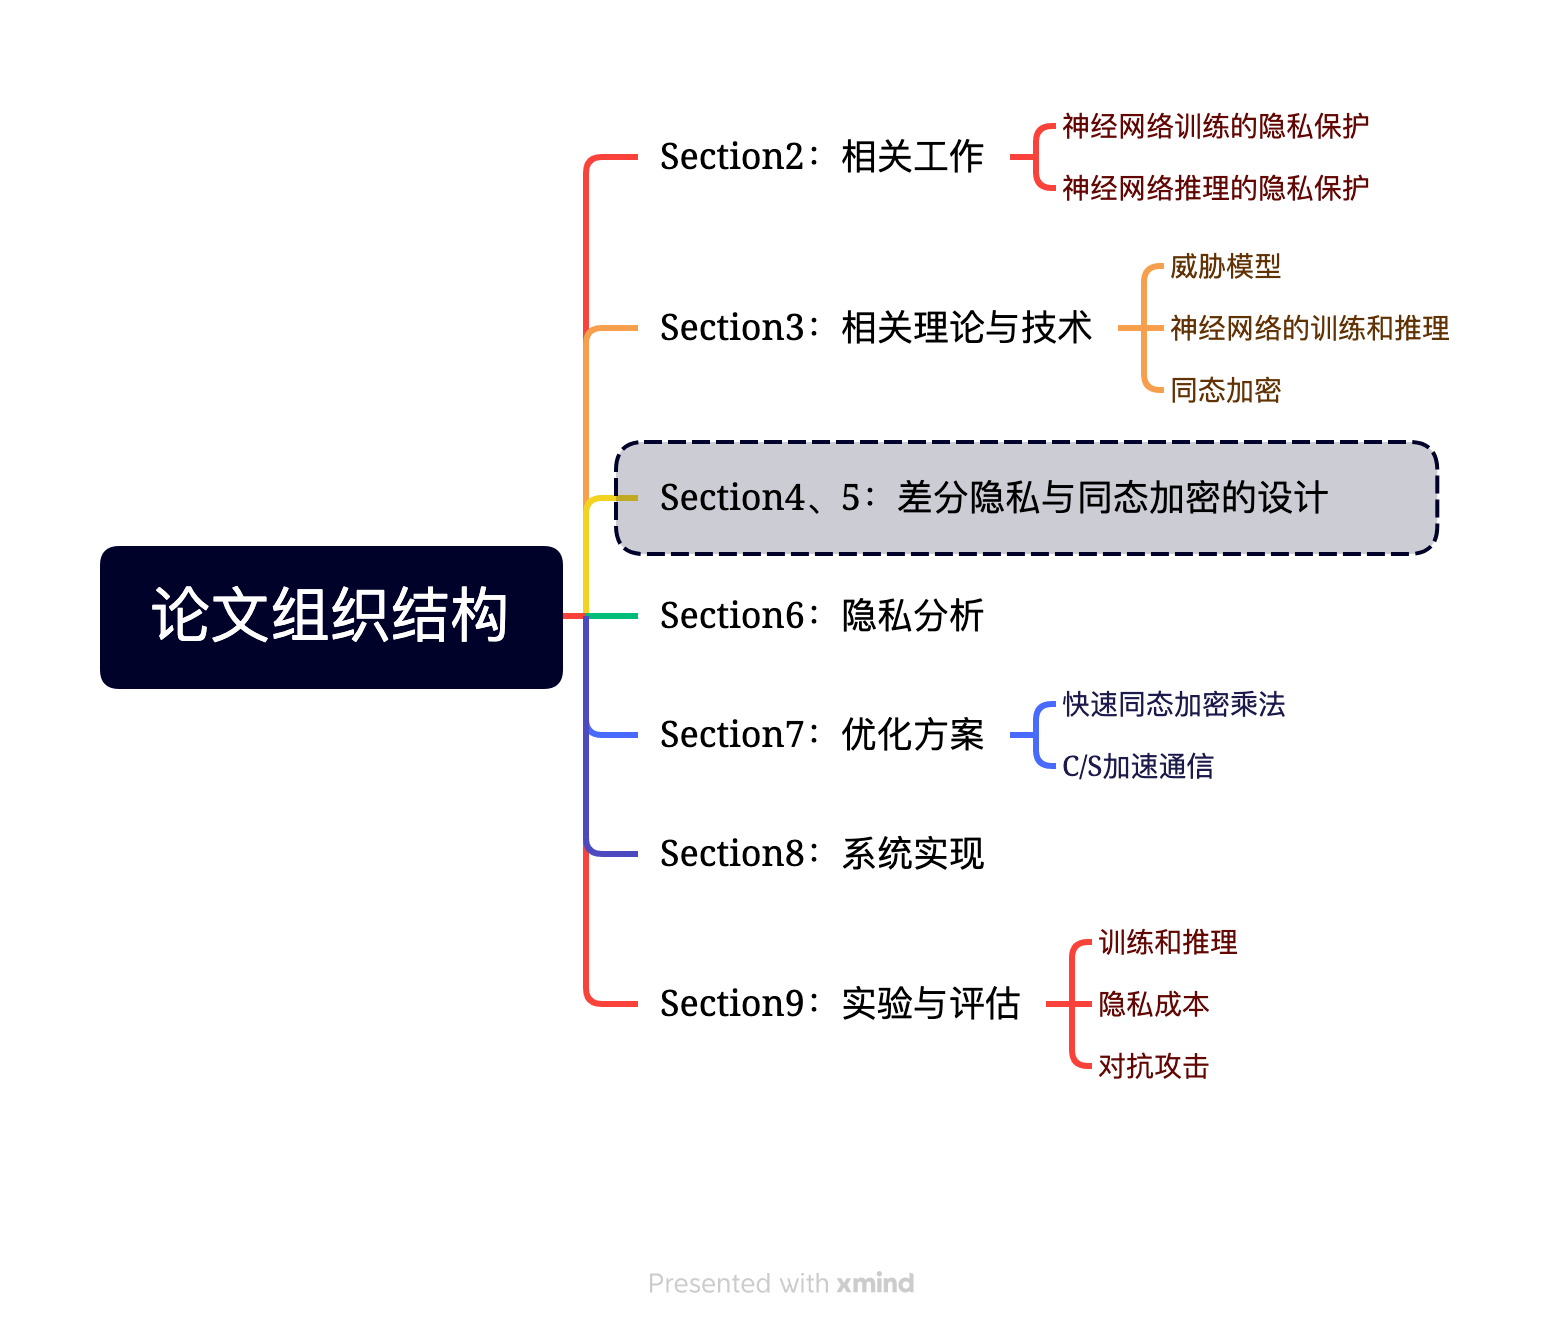
\includegraphics[height=.9\textheight]{pic/structure.png}
    \end{figure} 
\end{frame}


%%%%%%%%%%%%%%%%%%%%%%%%%%%%%%%%%%%%%%%%%%%%%%%%%%%%%%%%%%%%%%%%%%%%%%%%%%%
\section{研究背景与研究现状}
\subsection{同态加密与差分隐私技术}
\begin{frame}{同态加密与差分隐私技术}
\begin{exampleblock}{同态加密}
	背景:假设我有两个数$m_{1}$ 和$m_{2}$ ,我希望把它们扔给云计算平台做加法运算,但又不希望云计算平台知道$m_{1}$、$m_{2}$的值。设$m_1=100$, $m_2=200$,步骤如下:\\
	\begin{itemize}
		\item {\footnotesize(本地)生成一对钥匙,公钥pub和密钥priv,公钥用于加密,密钥用于解密。}
		\item {\footnotesize(本地)公钥pub分加密$m_{1}$和$m_{2}$,如:$E_{pub}(m_1)=1234$,$E_{pub}(m_2)=4321$}
		\item {\footnotesize (云计算平台)使用$Add_{pub}$函数对$E_{pub}(m_1)$和$E_{pub}(m_2)$进行计算,即:$Add_{pub}(1234, 4321)=12345678$}
		\item {\footnotesize (本地)使用密钥priv解密$Add_{pub}(1234, 4321)$,得到$D_{priv}(12345678) = 300$(严格意义上讲,是个近似值)。}
	\end{itemize}
\end{exampleblock}
\end{frame}
\begin{frame}{同态加密与差分隐私技术}
\begin{exampleblock}{差分隐私}
差分隐私是属于密码学的远亲,并没有使用传统意义上的加密解密,它是通过一种扰动的方法,对原始数据进行保护。(下面举一个简单例子,如有不当请指出)\\
\begin{itemize}
		\item {\footnotesize 假设有一个婚恋网站,系统只能够查询单身人数(有约束条件),攻击者的任务也是查找单身人数。}
		\item {\footnotesize 现在进行一次查询,发现系统有2人单身;然后张三跑去登记了,又进行一次查询发现系统显示3人单身。我们就可以推断出“张三单身”。在这里,张三作为一个样本的出现,让攻击者获得了奇怪的知识。{\color {red}而差分隐私要做的就是使攻击者获得的知识不会因为新样本的出现而发生变化。}}
		\item {\footnotesize 简单的差分隐私操作:添加噪声,第一次查询的时候显示2.5,第二次显示2.5,这样攻击者便不能判断张三是不是单身。}
	\end{itemize}

\end{exampleblock}
\end{frame}
\begin{frame}{同态加密与差分隐私技术}
\begin{exampleblock}{同态加密与差分隐私技术对比}
\begin{table}[htpb]
            \centering
            \caption{同态加密与差分隐私技术对比}
            \label{tab:number}
            \begin{tabular}{rcc}\toprule
            	隐私保护方案 & 同态加密 & 差分隐私 \\\midrule
            	隐私保护性 & 强 & 弱 \\
            	计算效率 & 慢(消耗计算资源) & 快 \\\bottomrule
            \end{tabular}
\end{table}
\begin{itemize}
		\item {\footnotesize 差分隐私:大多数是在模型中(或输出结果中)添加噪声,隐私保护能力不如同态加密;但是效率特别高,在隐私保护性要求不高的情况下用的比较多。}
		\item {\footnotesize 同态加密:效率比较低,非常消耗计算资源,但是隐私保护能力非常强。}

	\end{itemize}
\end{exampleblock}
\end{frame}




\subsection{现有的隐私保护方案}
\begin{frame}{现有的隐私保护方案}
	本文对现有的隐私保护方案进行归纳,可分为以下三种情况:
	\begin{itemize}
        \item {\footnotesize {\color {red}1)专注于推理阶段的隐私保护。}例如:\cite{liu2017oblivious}(CCS'17),MLaaS场景下用户要保护数据,服务商要保护模型。作者提出了一个两方计算框架MiniONN,将已经训练好的模型转化为一个不经意传输模型实现了数据和模型的保护。}
        \item {\footnotesize {\color {red}2)专注于训练阶段的隐私保护。}例如:\cite{nandakumar2019towards}(CVPR'19),作者评估了非交互式方式在加密数据上训练DNN的可能性,通过简化网络、选择图像合适的分辨率等技巧,提高了加密训练的效率。}
        \item {\footnotesize{\color {red}3)甚至是假设存在一个可信的中心或者多个非共谋的服务器。}例如:\cite{mohassel2017secureml}(SP'17),作者设计了2个半可信非共谋的服务器,交互执行密文下的计算。(作者认为这个假设是不现实的)。}
    	\end{itemize}
\end{frame}

\begin{frame}{现有的隐私保护方案}
	因此,作者提出了Sphinx:
	\begin{figure}[h]
    	\centering
        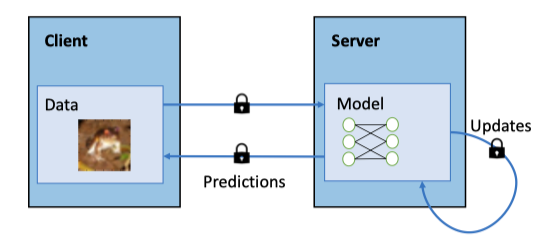
\includegraphics[height=.4\textheight]{pic/online-learning.png}
    \end{figure} 
	\begin{itemize}
        \item {\footnotesize 取消了他认为不现实的假设(作者认为:存在可信中心或者多个非共谋的服务器是不现实的),在本文中只有2方:用户(客户端)和服务商(服务端),没有可信的中心。}
        \item {\footnotesize 训练阶段的隐私保护、推理阶段的隐私保护都要兼顾。}
%        \item {\footnotesize \color{blue}提出一个小小的质疑:作者提出的场景,严格意义上说并不是MLaaS场景,而是一个PaaS场景。在该场景中,作者作为“用户”,既提供了自己的模型又使用了自己数据;而“服务商”只是提供了算力(用文中的话说,“提供了训练和推理的服务”),我认为只需要保护数据不被服务商窃取即可,至于模型的隐私好像不是那么重要(但文中保护了模型的参数,但没保护模型的结构)。}
    	\end{itemize}
\end{frame}
%%%%%%%%%%%%%%%%%%%%%%%%%%%%%%%%%%%%%%%%%%%%%%%%%%%%%%%%%%%%%%%%%%%%%%%%%%%
\section{算法设计}

%思路:
%1.训练过程
%2.卷积操作
%3.卷积神经网络的权重和偏置
%4.反向传播
%5.优化方案

\subsection{训练协议设计}
\begin{frame}{训练协议设计}
\begin{exampleblock}{设计思路:}
\begin{itemize}
		\item {\footnotesize 差分隐私通过添加噪声,在一定程度上可以起到保护隐私的作用(与纯明文比,是能保护隐私的)。}
		\item {\footnotesize 由于深度神经网络中涉及了大量的矩阵乘法运算,前人已有论证:完全使用同态加密算法进行计算,虽然隐私性强,但效率特别低。}
		\item {\footnotesize 而CKKS(本文使用的同态加密算法)支持明文与密文之间的混合操作,且要比密文与密文之间的运算耗费的计算资源少,效率要高。({\color {blue}求证:前面所述是在一篇技术分享里看到的一段话,待求证。})}
		\item {\footnotesize 因此,作者对隐私性做了“妥协”,不完全使用同态加密了,而是部分使用同态加密(偏置分量$b$),部分使用差分隐私(线性分量$\omega$)。}
		\item {\footnotesize {\color {blue}思考:是否可以对线性分量$\omega$进行同态加密,对偏置分量进行差分隐私?同态加密的加法和乘法,哪个效率更高?}}

	\end{itemize}
\end{exampleblock}
\end{frame}



\begin{frame}{训练协议设计}
\begin{exampleblock}{设计概览:}
本文假设神经网络模型是简单的分层结构,每层的公式为:\\
\begin{equation*}
f(x)=\sigma(W^Tx+b)
\end{equation*}
\\
其中,$\sigma$为非线性激活函数(以及池化操作),$W$为权重向量,$b$为偏置。
Sphinx使用同态加密对偏置$b$进行加密,使用差分隐私对权重$W$的计算进行扰动。协议的设计考虑了性能问题,此处如果完全使用同态加密,那计算速度会大打折扣。所以对于权重的计算仅使用了差分隐私的方案(明文)。
\end{exampleblock}
{\color {red} 热知识:非线性的激活函数可以提高模型的复杂度,但是同态加密无法处理非线性计算,因此非线性部分$f$是在用户端完成的。}
\end{frame}


\begin{frame}{训练协议设计}
    \begin{minipage}[l]{0.7\linewidth}
    \begin{exampleblock}{训练协议设计:初始化}
        	\begin{itemize}
    		\item {\footnotesize 用户:首先生成公钥私钥对$PK$和$SK$,并且将公钥$PK$以及初始模型结构发送给服务器;服务器:初始化模型参数$W^0$和$[b^0]$。}
    	\end{itemize}
    \end{exampleblock}
    \begin{exampleblock}{训练协议设计:训练过程}
        	\begin{itemize}
    		\item {\footnotesize 用户:采样数据,将样本加密得到$[x_i]$,然后将加密后的数据发送给服务器;服务器:服务器进行线性计算$W{_i}{^T}[x_i]+[b_i]$得到一个中间的密文,即为$[c_i]$,然后服务器将$[c_i]$发送给用户端进行解密;用户收到$[c_i]$后,进行如下计算:1)解密;2)非线性计算$f$;3)加密得到$[x_{i+1}]$;}
    	\end{itemize}
    \end{exampleblock}
   \end{minipage}
	%右侧
    \begin{minipage}{0.2\linewidth}
        \begin{figure}[h]
            \centering
%            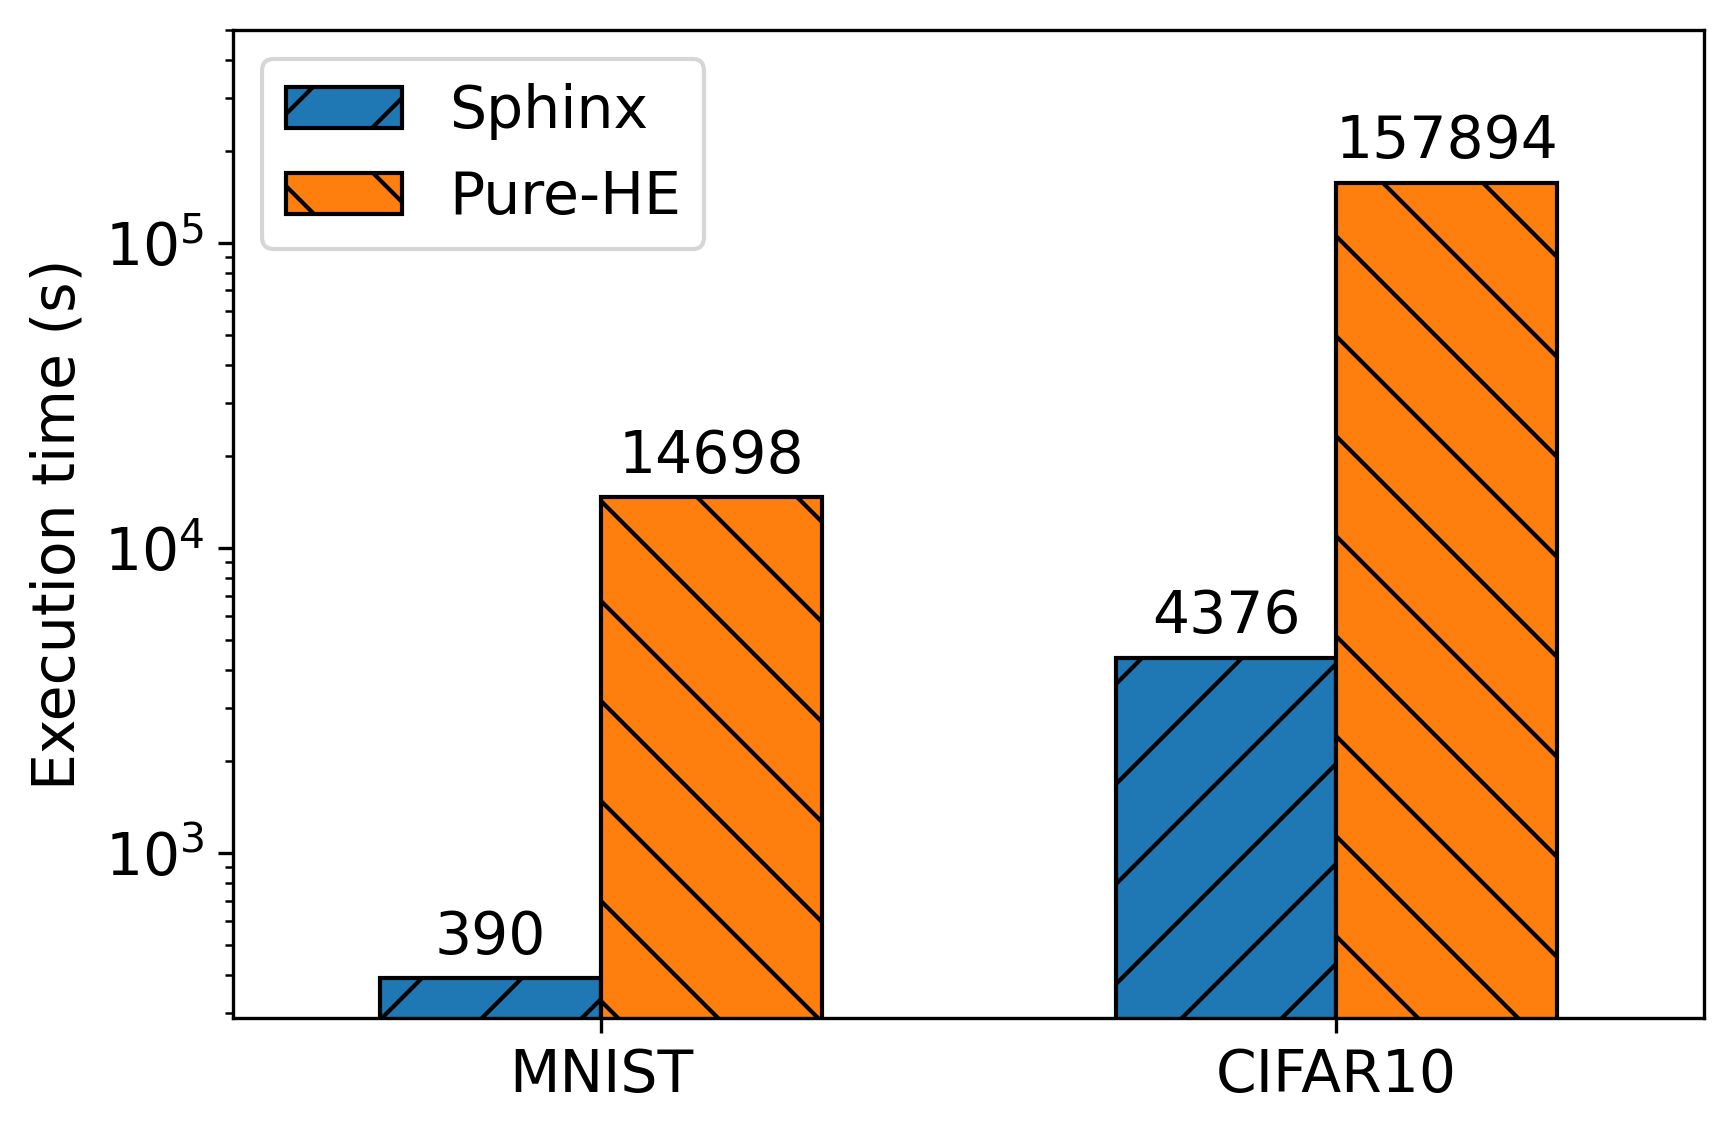
\includegraphics[height=.3\textheight]{pic/fig6.png}
             \hspace{2cm}
            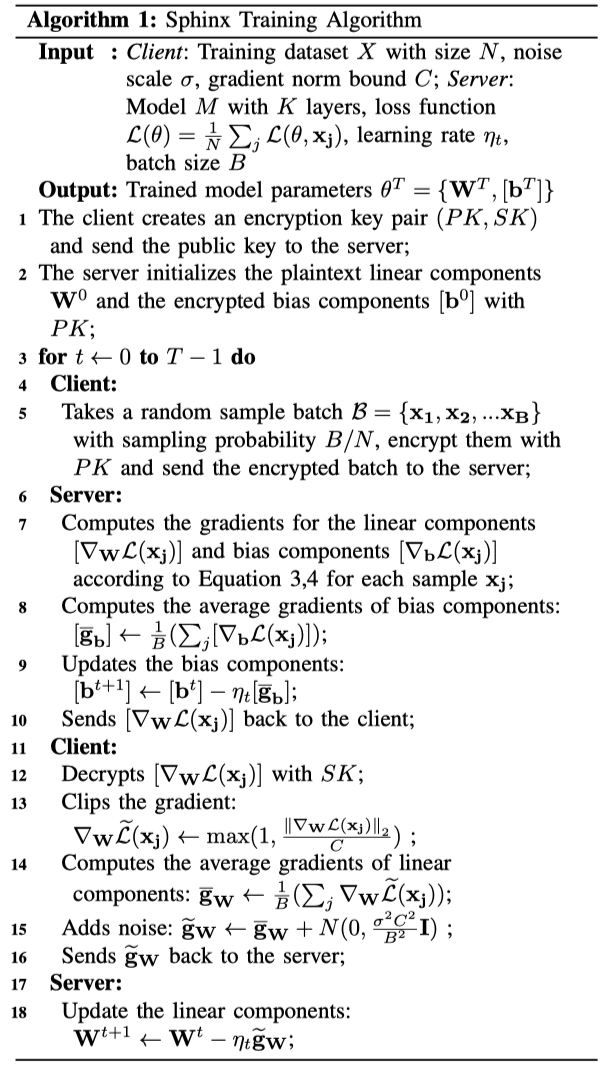
\includegraphics[height=.8\textheight]{pic/algorithm1.png}
        \end{figure} 
    \end{minipage}
\end{frame}

\begin{frame}{训练协议设计}
    \begin{minipage}[l]{0.7\linewidth}
    \begin{exampleblock}{训练协议设计:训练过程}
        	\begin{itemize}
    		\item {\footnotesize {\color {blue}疑问:对输入样本$[x_i]$的加密是用的什么算法?}}
    		\item {\footnotesize 优化:反向传播时,需要用到f的一阶导数。为了减少通信量,在进行非线性计算时便计算了激活函数$f$的导数,跟数据一起发送给服务器并缓存起来。}
    	\end{itemize}
    \end{exampleblock}
    \begin{exampleblock}{训练协议设计:更新过程}
        	\begin{itemize}
    		\item {\footnotesize 偏置单元$b$:服务器中本身拥有的就是加密版本(同态加密),直接更新到模型中。}
    		\item {\footnotesize 线性单元$W$:服务器将线性单元的梯度发送给用户,用户解密后添加噪声再给服务器,服务器更新模型(差分隐私)。}
    	\end{itemize}
    \end{exampleblock}
   \end{minipage}
	%右侧
    \begin{minipage}{0.2\linewidth}
        \begin{figure}[h]
            \centering
%            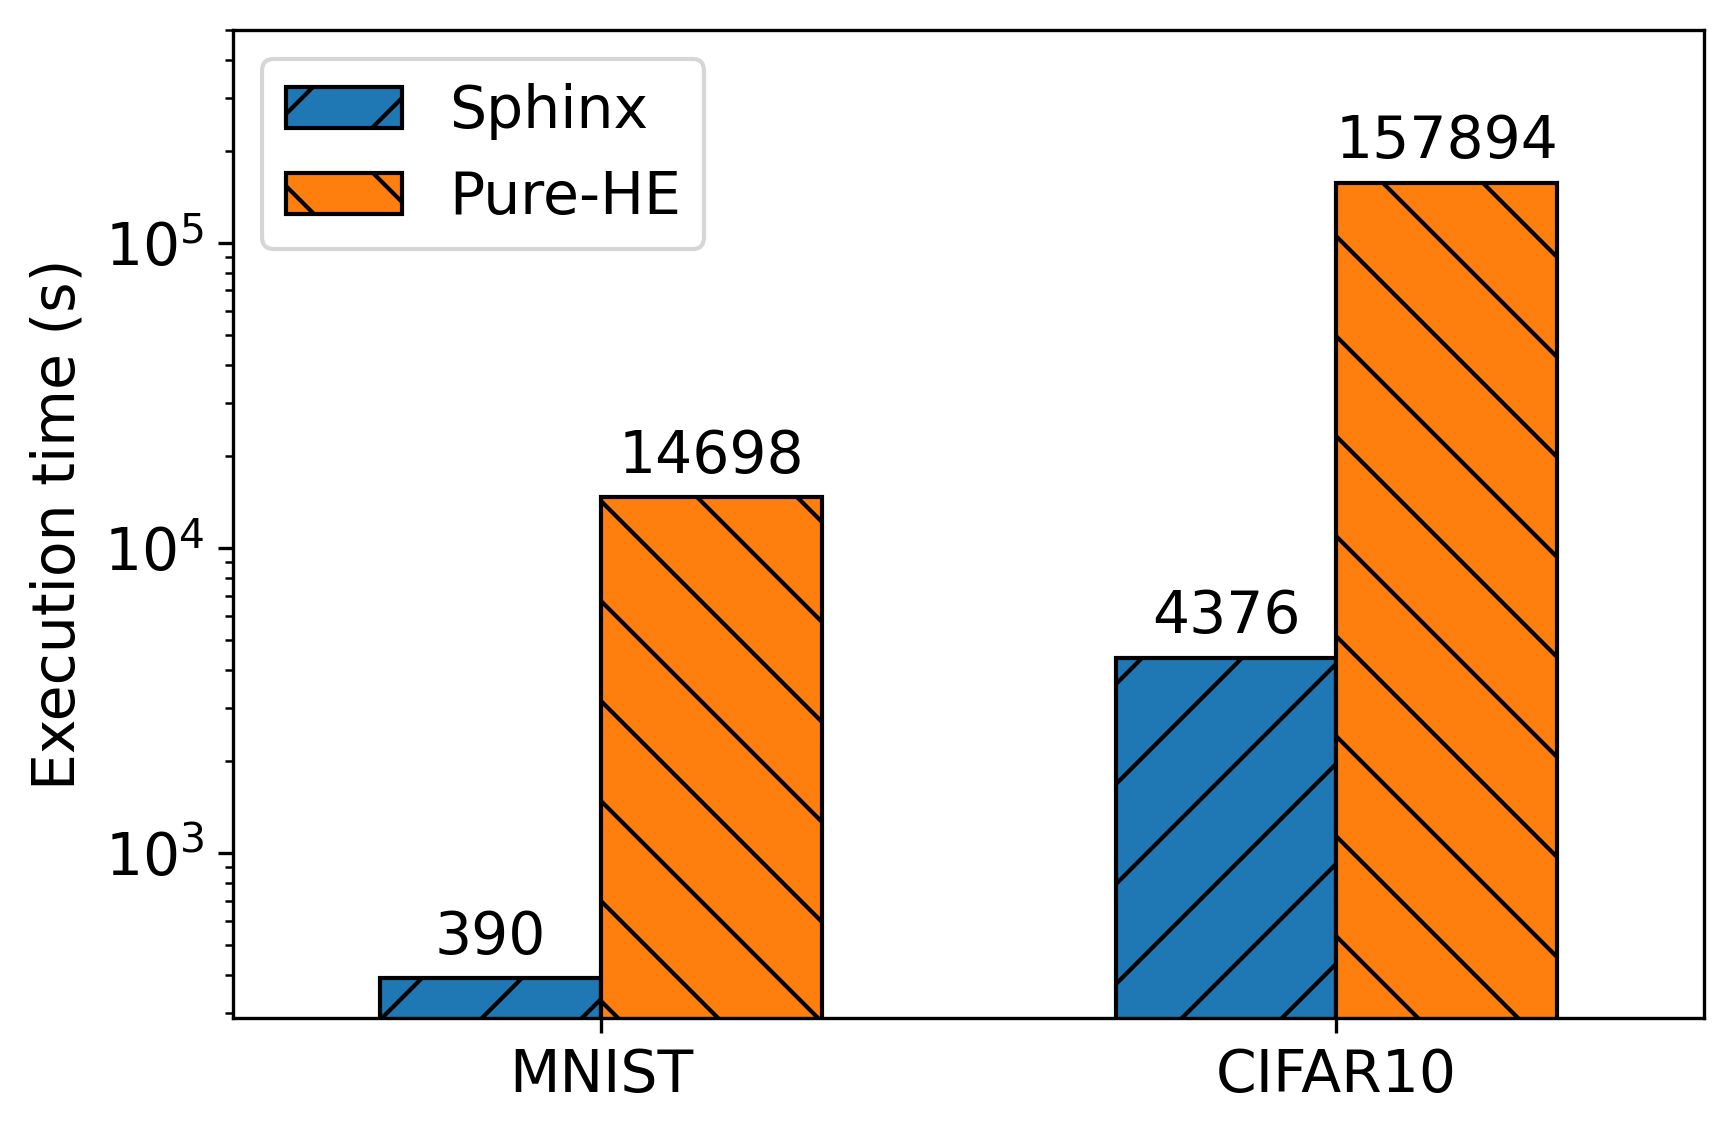
\includegraphics[height=.3\textheight]{pic/fig6.png}
             \hspace{2cm}
            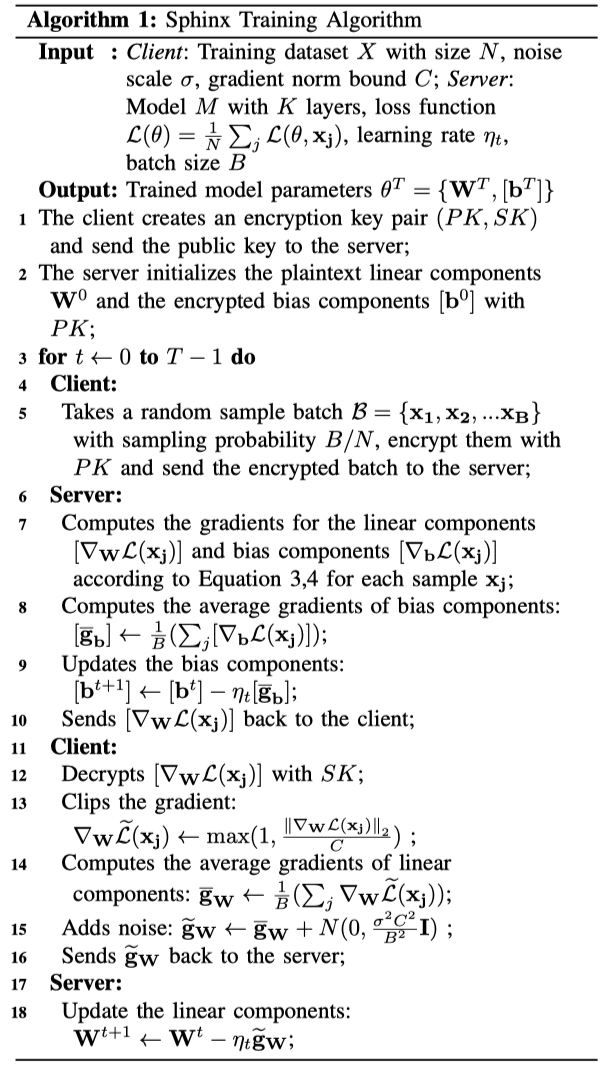
\includegraphics[height=.8\textheight]{pic/algorithm1.png}
        \end{figure} 
    \end{minipage}
\end{frame}



\subsection{推理协议设计}
\begin{frame}{推理协议设计}
    \begin{exampleblock}{推理协议设计:单个共享密钥($P_i$)生成过程}
    思想:推理阶段,不再用复杂的同态加密、解密操作。
%    为了保证推理服务的性能,论文涉及了一个优化方案:通过预处理阶段率先计算出很多个共享密钥(每次推理使用一个不同的共享密钥),来避免推理耗时的同态加密操作。
        	\begin{itemize}
    		\item {\footnotesize 用户:对每一层神经网络的输入生成一个mask向量$r_i$,服务器:为每一层神经网络的输出生成一个mask向量$s_i$,其中$i$是第$i$个线性层。}
    		\item {\footnotesize 用户:使用同态加密的方式对$r_i$进行加密,发送$[r_i]$给服务器。}
    		\item {\footnotesize 服务器:把加密后的$[r_i]$当做一个样本,计算$W{_i^T} \cdot [r_i] + [b_i] - s_i\longrightarrow [W{_i^T} \cdot r_i + b_i - s_i ]$,并将结果发送给用户。}
    		\item {\footnotesize 用户:解密得到:$P_i=W{_i^T} \cdot r_i + b_i - s_i$。}
    		\item {\footnotesize {\color {blue} 疑问:没明白mask向量$r_i$和$s_i$是怎么得到的。}}
    	\end{itemize}
    \end{exampleblock}
\end{frame}


\begin{frame}{推理协议设计}
    \begin{exampleblock}{推理协议设计:样本$X$推理过程}
        	\begin{itemize}
    		\item {\footnotesize 用户:预先挑选一个计算好的mask向量$r_i$,计算$x-r_i$,并将$x-r_i$发送给服务器。}
    		\item {\footnotesize 服务器:计算$W{_i^T} \cdot (x-r_i) + s_i$,并将结果发送给用户。}
    		\item {\footnotesize 用户:将计算的结果$W{_i^T} \cdot (x-r_i) + s_i$与之前的$P_i=W{_i^T} \cdot r_i + b_i - s_i$相加,得到$W{_i^T} \cdot x + b_i$}
    		\item {\footnotesize 部分参数抵消,直接获得推理的结果,$r_i$起到了保护样本$x$的作用,但不涉及加密解密操作。}
    	\end{itemize}
    \end{exampleblock}
\end{frame}




%\subsection{优化方案}

%%%%%%%%%%%%%%%%%%%%%%%%%%%%%%%%%%%%%%%%%%%%%%%%%%%%%%%%%%%%%%%%%%%%%%%%%%%
\section{实验与分析}
\subsection{实验环境设置}
\begin{frame}{实验环境设置}
\begin{table}[htpb]
            \centering
            \caption{实验环境设置}
            \label{tab:number}
            \begin{tabular}{rc}\toprule
                实验环境 & 具体配置及参数 \\\midrule
                物理机数量 & 2台(客户端和服务端)\\
                物理机CPU & 至强E5-2683CPU,128G内存\\
                操作系统 & Ubuntu18.04LTS\\
                网络环境 & 通过10Gbps局域网连接 \\
                编程语言 & C++、SEAL3.6(同态加密库)\\\bottomrule
%                数据集 & MNIST、CIFAR-10\\
            \end{tabular}
\end{table}
\begin{itemize}
	\item {\footnotesize 科普:10Gbps,万兆带宽,大约每秒能传输1G多的数据。}
	\item {\footnotesize \color{blue} 疑问:未提到GPU,是GPU不支持还是忽略了GPU?(不同算力效果是不一样的。)}
	\item {\footnotesize \color{blue} 质疑:1)目前广域网只普及到千兆级别,万兆尚未普及。2)若MLaaS部署在局域网,那就“不需要”考虑隐私保护了。}
\end{itemize}  
\end{frame}

\begin{frame}{实验环境设置}
\begin{table}[htpb]
            \centering
            \caption{模型参数设置}
            \label{tab:number}
            \begin{tabular}{rcc}\toprule
            	模型参数 & MNIST模型 & CIFAR-10模型 \\\midrule
            	batch size & 500 & 2000 \\
            	优化算法 & 随机梯度下降(SGD) & 随机梯度下降(SGD) \\
            	学习率 & 0.1 & 0.05 \\\bottomrule
            \end{tabular}
\end{table}
\begin{itemize}%[<+-| alert@+>]
	\item {\footnotesize MNIST数据集(0-9共10个分类),主要用于分类任务;CIFAR-10(共10个分类),也主要用于分类任务,与MNIST数据集不同的是,CIFAR-10数据集是彩色图像。}
	\item {{\footnotesize \color {red}实验结果:作者在MNIST和CIFAR-10数据集上得到的最佳准确率(Accuracy)分别为98.5\%和78.8\%}}。
\end{itemize}  
\end{frame}



\subsection{神经网络结构}
\begin{frame}{神经网络结构}
\begin{figure}[h]
    	\centering
        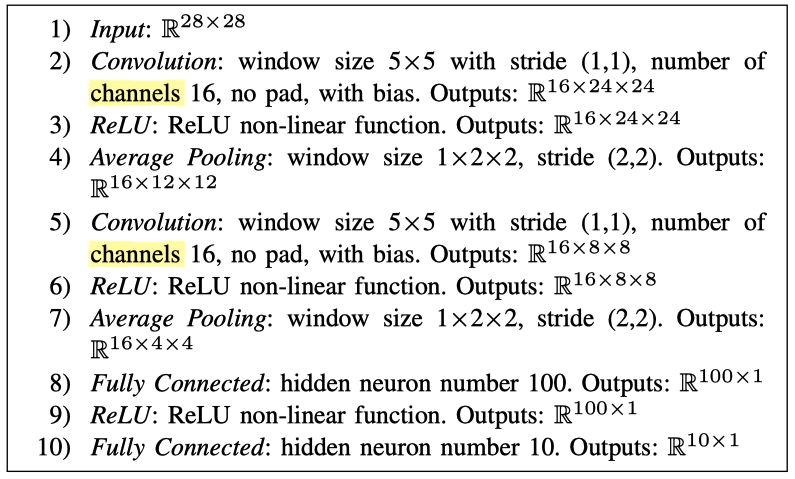
\includegraphics[height=.7\textheight]{pic/fig4.png}
\end{figure} 
    
\begin{itemize}
\item {\footnotesize 卷积核的通道数=输入的通道数}
\item {\footnotesize 卷积核的数量=输出的通道数}
\end{itemize}
\end{frame}


\subsection{实验结果分析}
\begin{frame}{模型训练实验分析}
	% 左侧	
    \begin{minipage}[l]{0.7\linewidth}
    \begin{exampleblock}{1.训练时间对比分析}
        	\begin{itemize}
    		\item {\footnotesize 右图为Sphinx和纯同态加密算法(Pure-HE)在1个batch上训练时间的比较,从图中可以看出,Sphinx比Pure-HE的训练时间减少了35倍(在MNIST数据集上的训练时间减少了36.68倍,在CIFAR-10上减少了35.08倍)。}
    		\item {\footnotesize 注:Pure-HE整个模型都是加密的,所有的同态运算发生在密文与密文之间。而Sphinx由于只对偏置单元$b$进行了加密,所以是密文与明文之间的同态运算。}
    	\end{itemize}
   \end{exampleblock}
   \end{minipage}
	%右侧
    \begin{minipage}{0.2\linewidth}
        \begin{figure}[h]
            \centering
            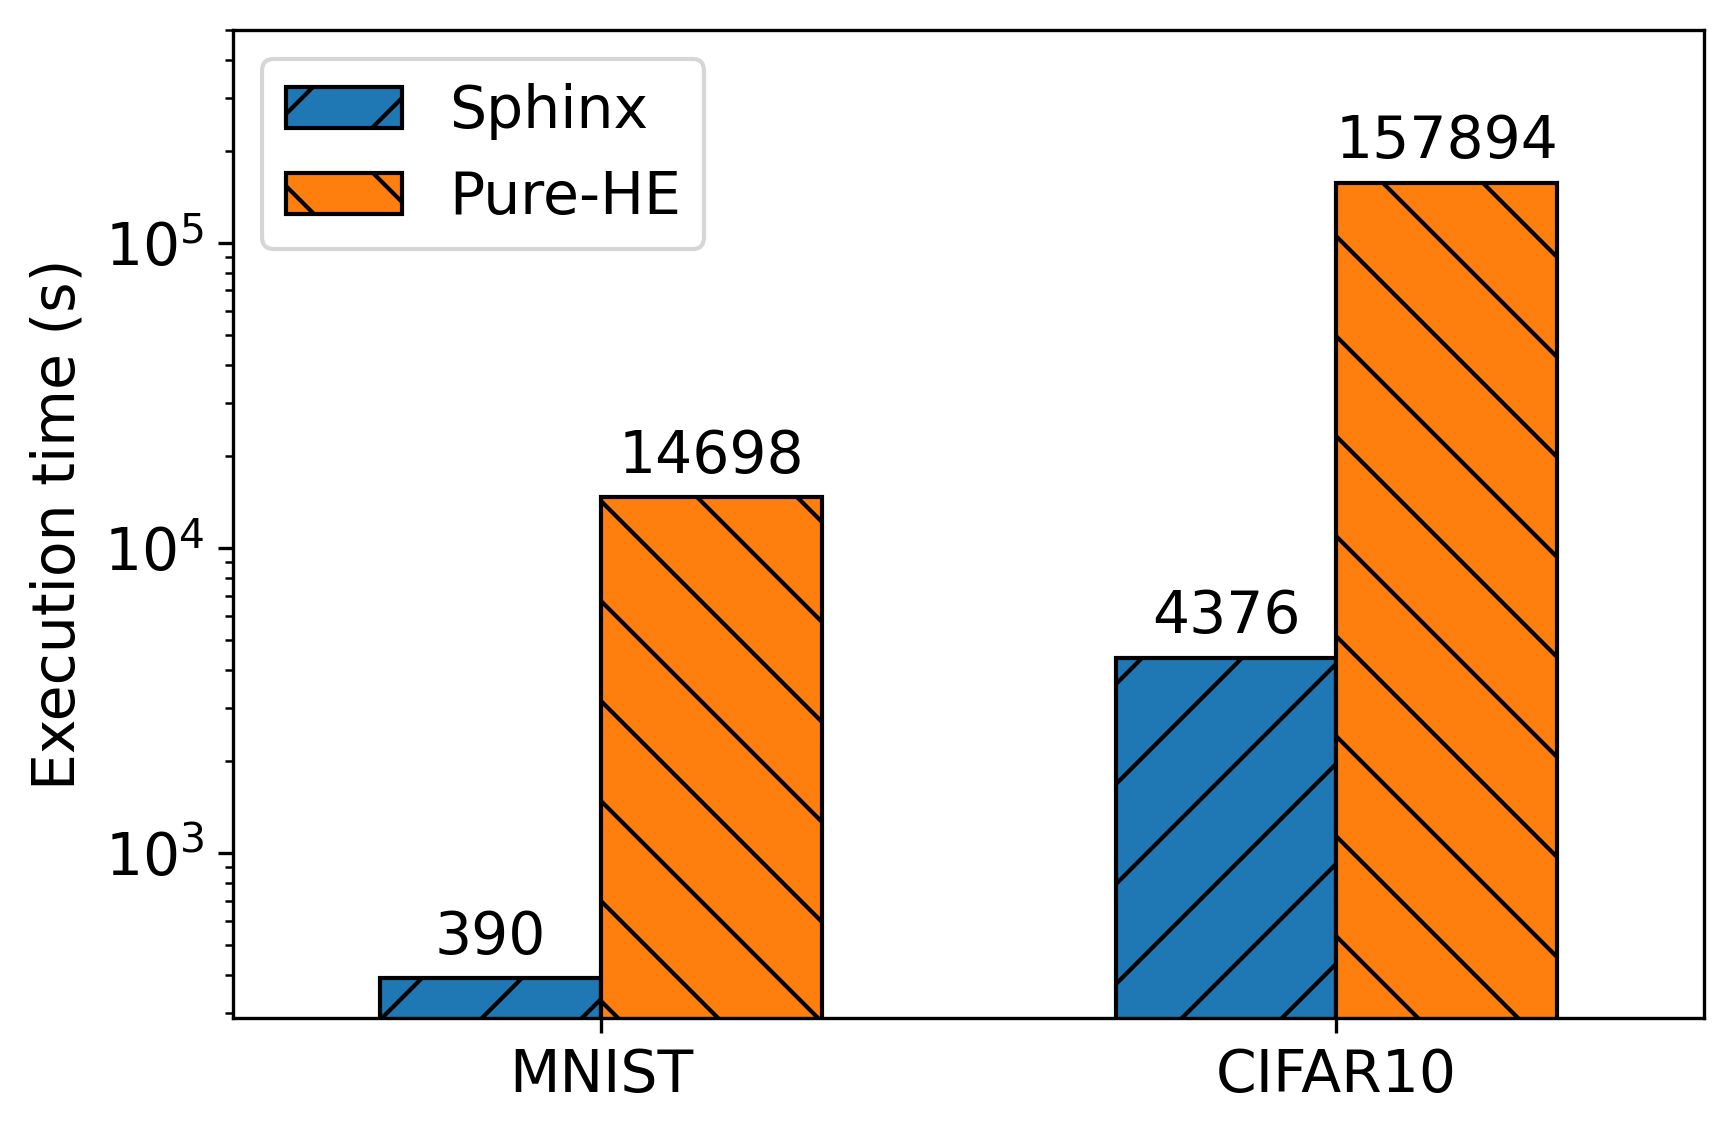
\includegraphics[height=.3\textheight]{pic/fig6.png}
             \hspace{2cm}
%            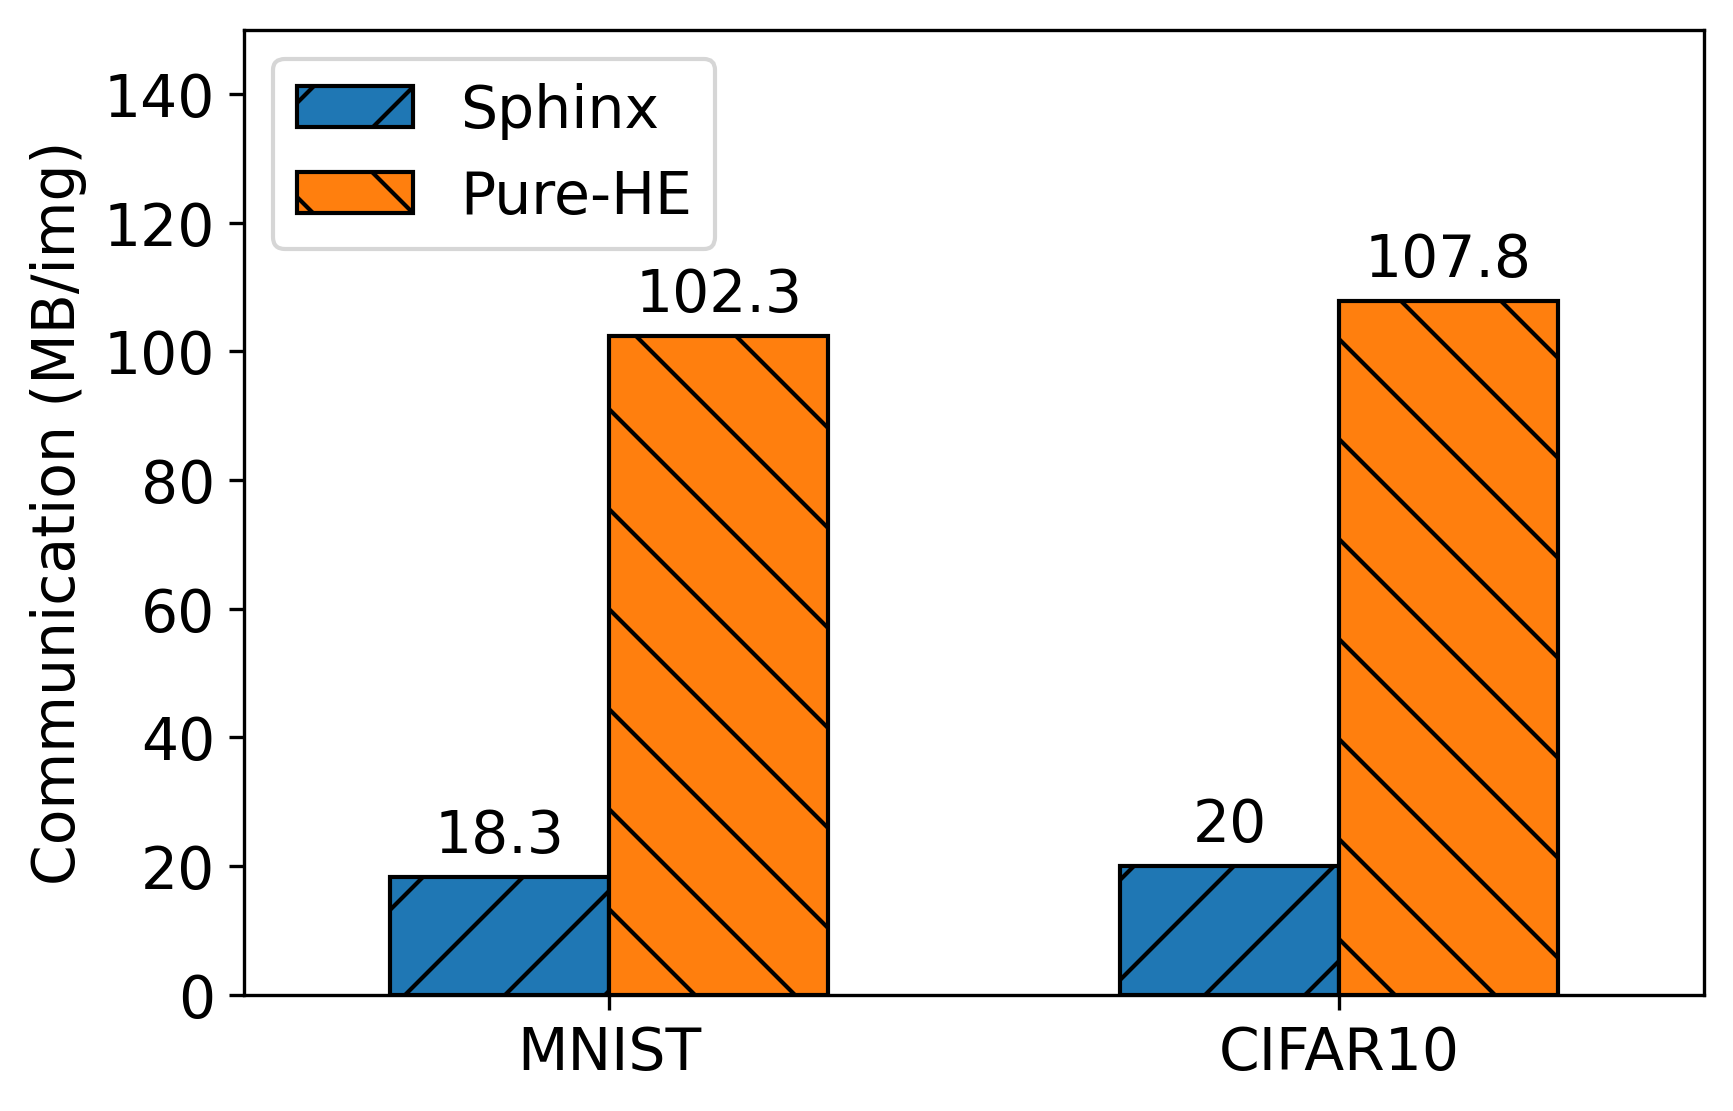
\includegraphics[height=.3\textheight]{pic/fig7.png}
        \end{figure}  
    \end{minipage}
\end{frame}

\begin{frame}{模型训练实验分析}
    \begin{minipage}[l]{0.7\linewidth}
    \begin{exampleblock}{2.通信开销对比分析}
        	\begin{itemize}
    		\item {\footnotesize 右图为Sphinx和纯同态加密算法(Pure-HE)在1个batch上通信开销的比较,从图中可以看出,Sphinx比Pure-HE的通信开销减少了5倍。}
    		\item {\footnotesize 原因分析:Sphinx通过保护线性分量为明文,避免了大多数繁重的同态操作(如:密文与密文矩阵乘法、缩放和重线性化)}
    		\item {\footnotesize \color{blue} 疑问:为什么训练时间和通信开销的对比分析实验中使用的是batch而不是epoch?(引发部署可行性的思考)【注意:接下来本人要闹笑话了!】}
    	\end{itemize}
    \end{exampleblock}
   \end{minipage}
	%右侧
    \begin{minipage}{0.2\linewidth}
        \begin{figure}[h]
            \centering
%            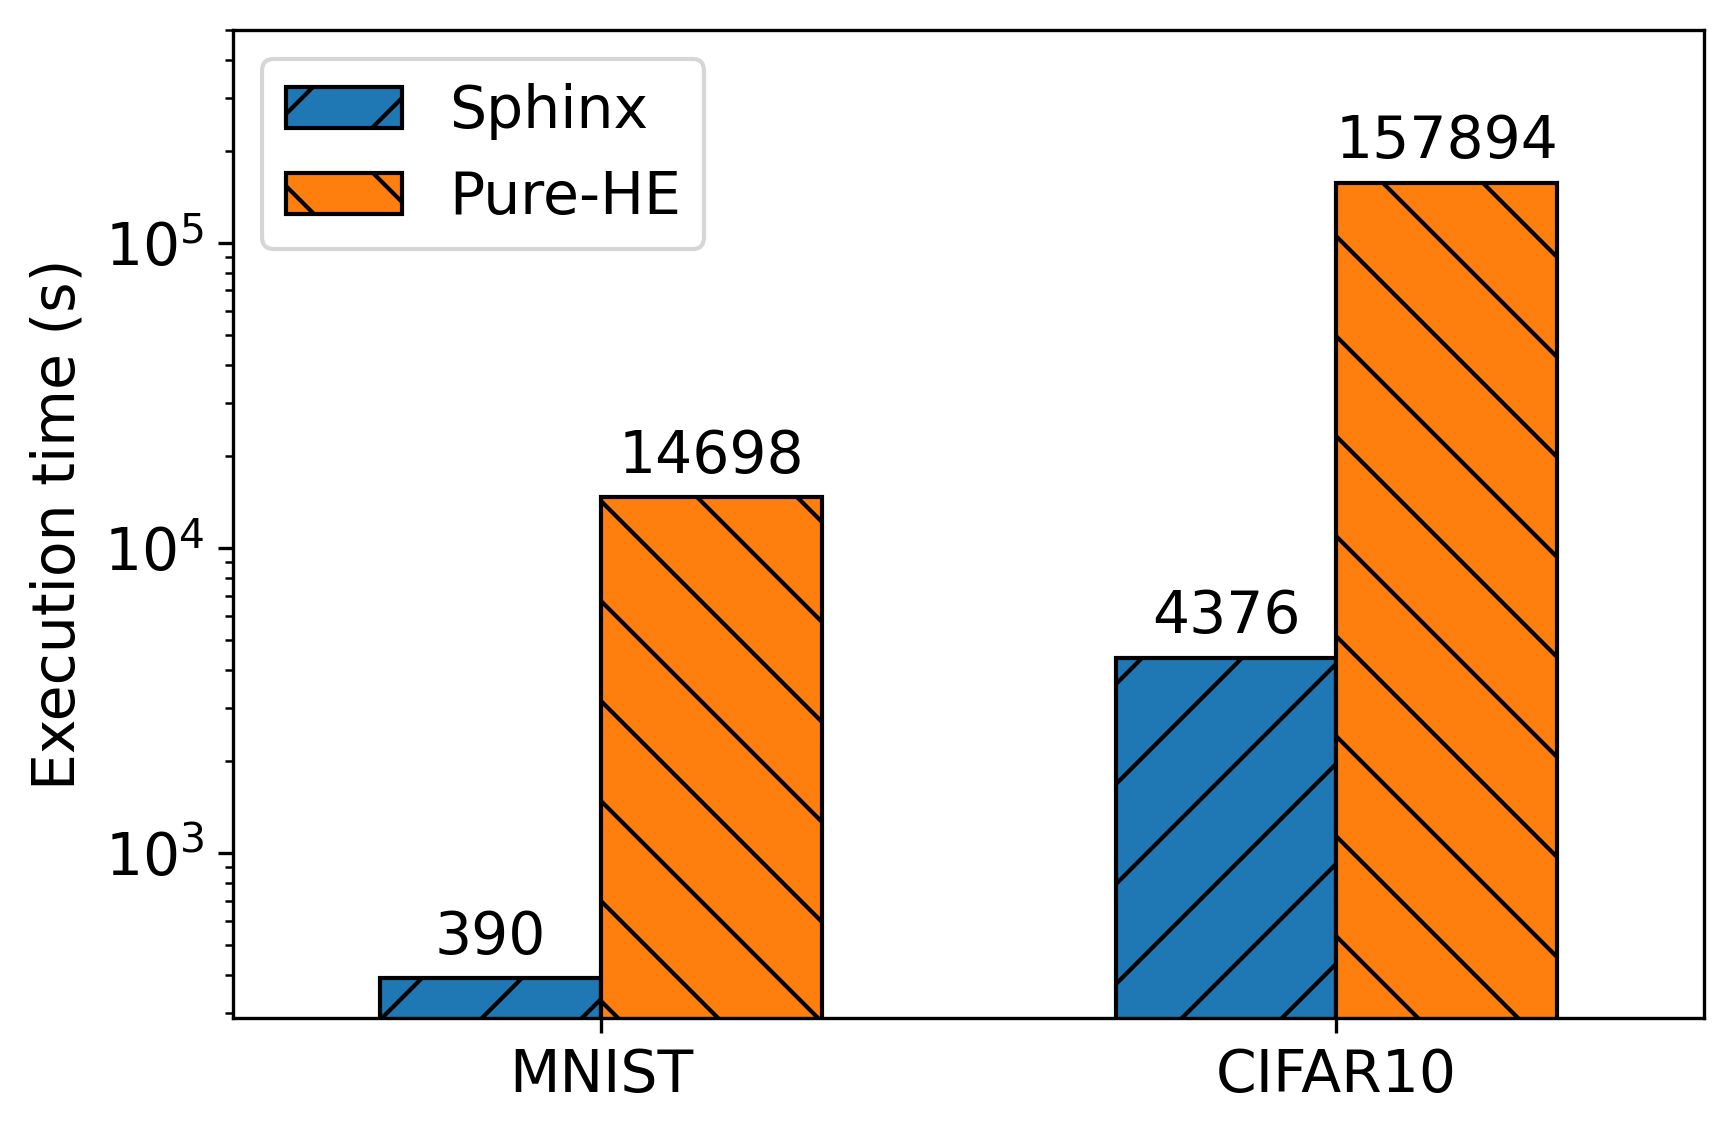
\includegraphics[height=.3\textheight]{pic/fig6.png}
             \hspace{2cm}
            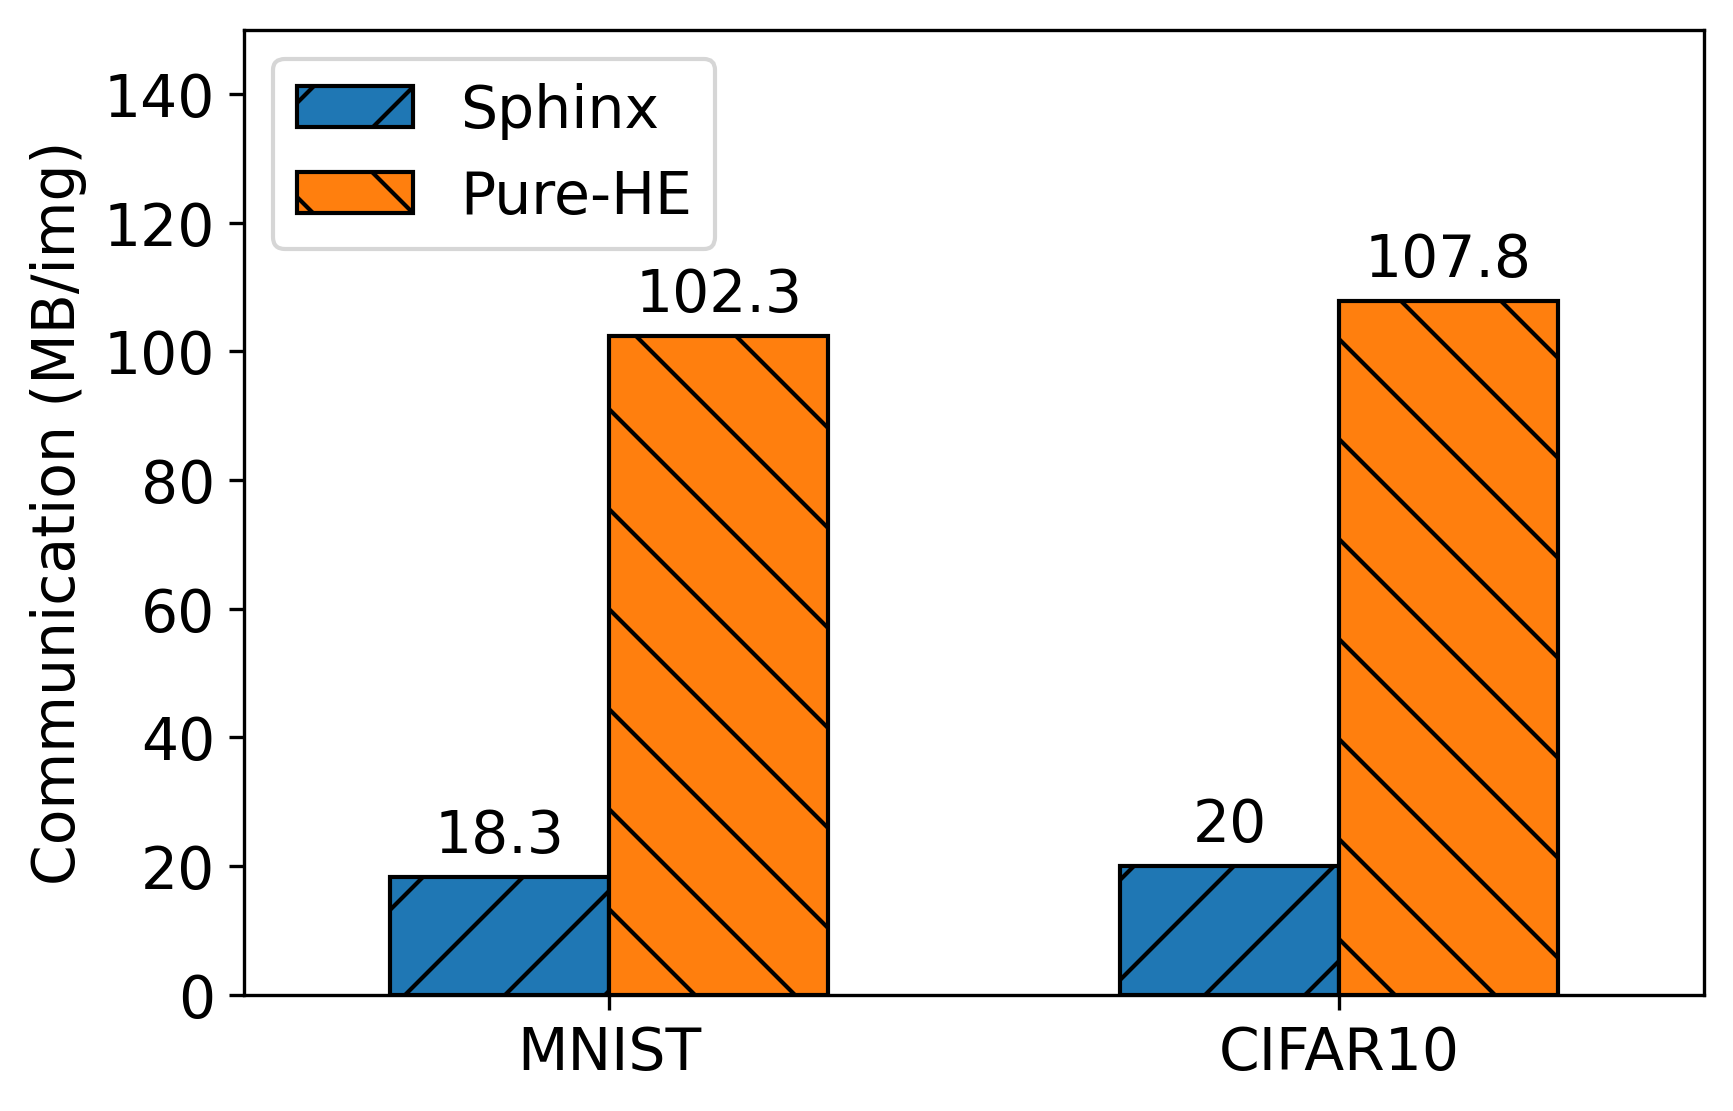
\includegraphics[height=.3\textheight]{pic/fig7.png}
        \end{figure} 
    \end{minipage}
\end{frame}



\begin{frame}{部署可行性的思考}	
\begin{exampleblock}{相关名词}
	\begin{itemize}
        \item {\footnotesize epoch:训练的轮数,1 epoch 指所有样本都经过了1次训练;batch:参数更新是分批进行的,1批就是1个batch,1批训练完称为 1 iteration(迭代);batch-size:每个batch中样本数量。}
        \item {\footnotesize 例如:MNIST训练集中有60000张图片,作者设置的batch size为500。指60000张图片分成了120批(batch=120),每批有500张(batch size=500),训练完1批称为1次迭代(iteration+1)。}
    	\end{itemize}
    \end{exampleblock}
\begin{exampleblock}{可行性思考}
	\begin{itemize}
        \item {\footnotesize 如果390s是指的“1 epoch的时间”,推论:勉强能用(i7CPU+3060单卡+本机+Resnet50模型1个epoch约370s);如果390s是指的“1 iteration的时间”,推论:无法实际部署(上述低配版3.12s)}
    	\end{itemize}
    \end{exampleblock}
\end{frame}


%%%%%%%%%%%%%%%%%%%%%%%%%%%%%%%%%%%%%%%%%%%%%%%%%%%%%%%%%%%%%%%%%%%%%%
\begin{frame}{模型推理实验分析}
\begin{minipage}[l]{0.6\linewidth}
右图为单个样本的推理延迟、通信开销,结论如下:
\begin{itemize}
	\item {\footnotesize 与Pure-HE相比Sphinx-FP推理延迟减少了近30倍,通信成本减少了近4倍,但由于同态操作,推理延迟和通信成本仍然很高。}
	\item {\footnotesize 然而,Sphinx与Pure-HE比,实现了更低的推理延迟($5.8\cdot10^4$和$4.2\cdot10^5$倍)和通信开销($1.9\cdot10^5$和$3.6\cdot10^4$),可以与最先进的方法Delphi媲美。}
	\item {\footnotesize 但Delphi和Gazelle等私有推理协议需要公共模型,因此不适用于在线学习。}
\end{itemize}
\end{minipage}
\begin{minipage}[l]{0.3\linewidth}
    \begin{figure}[h]
            \centering
             \hspace{2cm}
            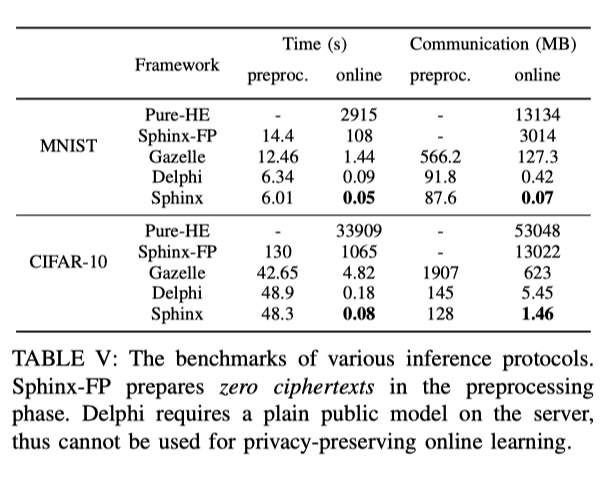
\includegraphics[height=.5\textheight]{pic/table5.png}
        \end{figure} 
\end{minipage}
\end{frame}



%\begin{frame}{隐私性分析}
%\begin{figure}[h]
%\centering
%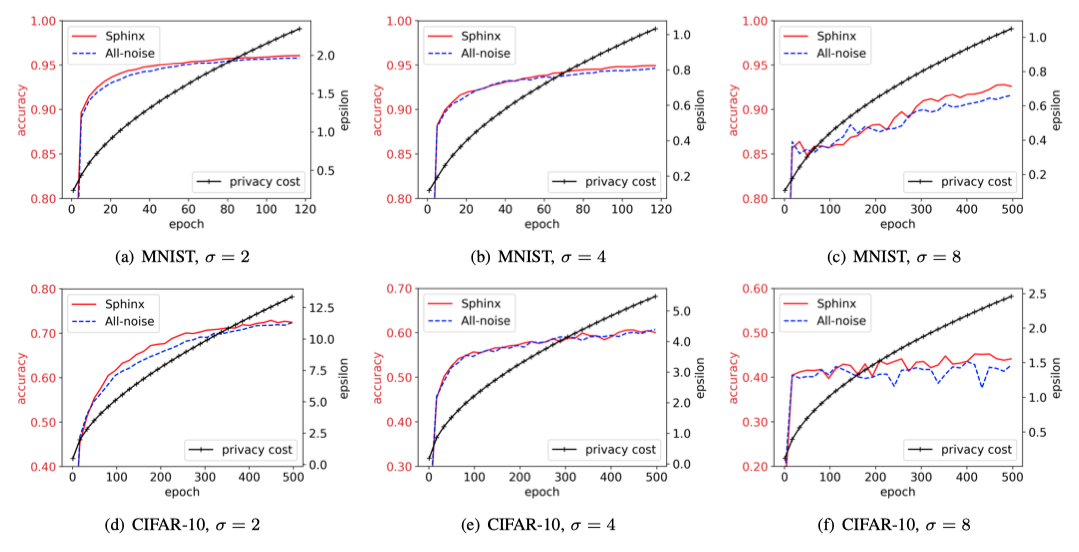
\includegraphics[width=8cm]{pic/fig8.png}
%\end{figure}

% {\footnotesize 本文在不同的噪声水平上($\delta$=2,4,8)进行实验。图中显示了随着训练的进行,Sphinx和全噪声算法准确性和隐私成本的变化。作者观察发现,噪声较大时,训练过程消耗的隐私预算较慢,这会导致学习不稳定,影响收敛速度。CIFAR-10的差分隐私模型的准确率下降的比MNIST要大。主要原因是CIFAR-10数据量大,任务复杂,而且神经网络层次越深,参数越多。(但是由于神经网络的可解释性较差,如何根据任务、数据集选择合适的模型架构,噪声水平、以及范数边界)}

%\end{frame}
%%%%%%%%%%%%%%%%%%%%%%%%%%%%%%%%%%%%%%%%%%%%%%%%%%%%%%%%%%%%%%%%%%%%%%



\begin{frame}{对抗攻击分析}
\begin{figure}[h]
\centering
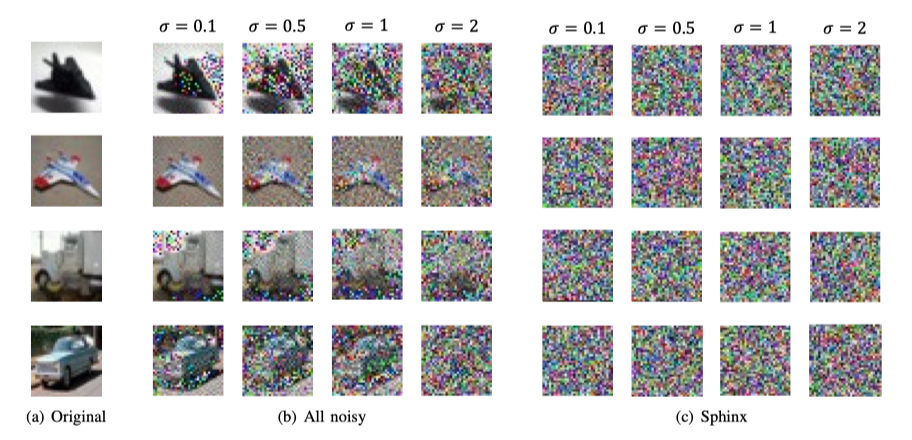
\includegraphics[height=.6\textheight]{pic/fig9.png}
\end{figure}
{\footnotesize 为了评估Sphinx在实际场景中对已知攻击的防御效果,作者进行了梯度匹配攻击(梯度匹配攻击\cite{zhao2020idlg}是一种利用模型的梯度恢复输入图像和标签的攻击方法)。实验结果表明:Sphinx模型防御梯度匹配攻击能力更强。
}
\end{frame}



%%%%%%%%%%%%%%%%%%%%%%%%%%%%%%%%%%%%%%%%%%%%%%%%%%%%%%%%%%%%%%%%%%%%%%%%%%%

\section{总结}
\begin{frame}{总结}	
\begin{exampleblock}{本文的优点}
	\begin{itemize}[<+-| alert@+>]
        \item {\footnotesize 取消了不现实的假设,同时考虑了训练、推理两阶段的隐私保护问题(数据隐私和模型参数隐私)。}
        \item {\footnotesize 题目吸引读者,用Sphinx比喻了算法设计方案(此条为本人的推断)。}
        \item {\footnotesize 使用了CKKS的一些特性,对原始模型进行了优化,提高了计算效率,减小了通信开销;mask向量设计的很巧妙(但本人脑子懂了手没学会)。}
    	\end{itemize}
    \end{exampleblock}
\begin{exampleblock}{本文的缺点}
	\begin{itemize}[<+-| alert@+>]
        \item {\footnotesize 文章的组织结构不是很喜欢,导致阅读困难。}
        \item {\footnotesize 文章中部分涉及深度学习的知识出现码字错误。}
        \item {\footnotesize 实验不太严谨,训练过程的实验环境与隐私保护场景相违背。}
    	\end{itemize}
    \end{exampleblock}
\end{frame}




\section{参考文献}
% allowframebreaks 是允许跨页
\begin{frame}[allowframebreaks]{参考文献列表}
    \bibliography{ref}
%    \bibliographystyle{alpha}
    % 如果参考文献太多的话,可以像下面这样调整字体:
    \tiny \bibliographystyle{alpha}
\end{frame}



% 致谢页
%\section{致谢}
\begin{frame}
    \begin{center}
        {\Huge\calligra 感谢各位的聆听}
    \end{center}
    
\end{frame}

\end{document}